\documentclass[border=5pt]{standalone}
\usepackage[T1]{fontenc}
\usepackage{lmodern,amsmath}
\usepackage{pgfplots}
\pgfplotsset{compat=1.18}
\begin{document}
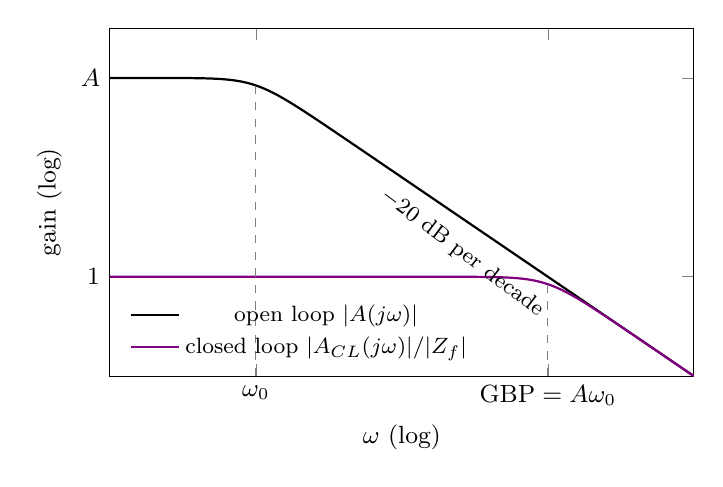
\begin{tikzpicture}[font=\small]
\begin{loglogaxis}[width=9cm,height=6cm,
  xmin=1e-2,xmax=1e6,ymin=1e-2,ymax=1e5,
  xtick={1,1e4},xticklabels={$\omega_0$,$\mathrm{GBP}=A\omega_0$},
  ytick={1,1e4},yticklabels={$1$,$A$},
  xlabel={$\omega$ (log)},ylabel={gain (log)},
  legend style={at={(0.02,0.02)},anchor=south west,draw=none,fill=none,font=\footnotesize},
  samples=200,domain=1e-2:1e6]
\addplot[black,thick] {1e4/sqrt(1+x^2)};
\addlegendentry{open loop $|A(j\omega)|$}
\addplot[violet,thick] {(1e4/(1+1e4))/sqrt(1+(x/(1+1e4))^2)};
\addlegendentry{closed loop $|A_{CL}(j\omega)|/|Z_f|$}
\draw[dashed,gray] (axis cs:1,1e-2) -- (axis cs:1,1e4);
\draw[dashed,gray] (axis cs:1e4,1e-2) -- (axis cs:1e4,1);
\node[font=\footnotesize,anchor=south west,rotate=-37] at (axis cs:30,30) {$-20$ dB per decade};
\end{loglogaxis}
\end{tikzpicture}
\end{document}
